\documentclass[11pt]{article}

% \usepackage{acl2016}

\usepackage{times}
\usepackage{latexsym}
\usepackage{color}
\usepackage{url}
\usepackage{wrapfig}
\usepackage{graphicx}
\def\UrlBreaks{\do\/\do-}
\usepackage{csvsimple}
\usepackage{arabtex}
\usepackage{utf8}
\usepackage{float}
\usepackage{coling2016}

\setcode{utf8}
% \setlength{\parindent}{4em}

% \aclfinalcopy % Uncomment this line for the final submission
% \def\aclpaperid{1} %  Enter the acl Paper ID here

% \title{Optimized Training and Evaluation of Arabic Word Embeddings}

% \author{Jordan King \and Lisa Singh\\
% 	    Georgetown University\\
% 	    3700 O Street NW\\
% 	    Washington, DC, 20057, USA\\
% 	    {\tt jwk67@georgetown.edu} \and\\
% 	    {\tt lisa.singh@cs.georgetown.edu}
% 	  \And
% 		Eric Wang \and David Buttler\\
% 	    Lawrence Livermore National Laboratory\\
% 	    7000 East Ave\\
% 	    Livermore, CA, 94550, USA\\
% 	    {\tt ericxwang.py@gmail.com} \and\\
% 	    {\tt buttler1@llnl.gov}
% 	    }

\title{Methods to Overcome Challenges When Learning Arabic Word Embeddings for Text Mining Tasks}
% \author{Jordan King}

\author{Jordan King \\
  Georgetown University / 3700 O st NW \\
  Georgetown University / Washington, DC \\
  Georgetown University / 20005 \\
  {\tt jwk67@georgetown.edu} \\\And
  Lisa Singh \\
  Georgetown University / 3700 O st NW \\
  Georgetown University / Washington, DC \\
  Georgetown University / 20005 \\
  {\tt lisa.singh@georgetown.edu} \\}
% \previousdegree{Computer Science Undergraduate}
% \thisdegree{Bachelor of Science}  % or Doctor of Philosophy, etc.
% \thisdiscipline{Computer Science}
% \thesistype{Senior Thesis}     % or Dissertation

% \thesisday{5}
% \thesismonth{May}
% \thesisyear{2016}
% \professor{Dr. Lisa Singh}
% \fulltitle{Methods to Overcome Challenges When Learning Arabic Word Embeddings for Text Mining Tasks}
% \indexwords{Arabic, Natural Language Processing, Word Embeddings, Word Vectors, Buzz, Text Mining}
% \dean{Ed Meyertholen}
% \memberi{Dr. Jeremy Fineman}
% \memberii{Calvin Newport}

\date{}

\begin{document}
% \pagenumbering{roman}
\maketitle   


% \tableofcontents
% \listoffigures 
% \listoftables  

% \newpage
% \pagenumbering{arabic}  % Ordinary pages have Arabic numerals.


\begin{abstract}
\label{sec:abstract}

Word embeddings are an increasingly important tool for NLP tasks that require semantic understanding of words. Little attention has been given to the production and application of Arabic word embeddings. Arabic is far more morphologically complex than English due to the many conjugations, suffixes, articles, and other grammar constructs. This has a significant effect on the training and application of Arabic word embeddings. While there are a number of techniques to break down Arabic words through lemmatization and tokenization, the quality of resulting word embeddings must be investigated to understand the effects of these transformations. In this paper, we investigate a number of preprocessing methods and training parameterizations to establish guideline methodologies for training high quality Arabic word embeddings. Using various evaluation tasks, including a new semantic similarity task created by fluent Arabic speakers, we are able to identify training strategies that produce high quality results for each task. To summarize, the main contributions of this work include improved methodologies for training Arabic word vectors, a semantic similarity task developed by native Arabic speakers, and a python package of Arabic text processing tools.

\end{abstract}
\section{Introduction}


Arabic word embeddings are numerical vector representations of a word's meaning - both semantic meaning and syntactic meaning. These embeddings are obtained using machine learning algorithms - word2vec - that utilize the context a word appears in to infer its meaning \cite{mikolovdist:2013, mikoloveffic:2013}. This works very well as words with similar meanings tend to be used in similar contexts, which are defined by the preceeding and following $n$ words. For example, the sentences \textit{I eat bread every night} and \textit{I eat rice every night} are examples of how food words may appear in similar contexts. With enough text to process, we can train numerical vectors to learn that bread and rice appear in these \textit{common-for-food} contexts. Similarly, we can learn syntactic relationships because different parts of speech appear in certain context patterns as well.
\\
High quality word embeddings provide a representation of the meaning of a word, without ever translating or referencing a dictionary. We can obtain the semantic and syntactic meaning directly from a corpus of natural written language. With accurate word embeddings, we can perform powerful vector operations to investigate the relationships between words in a corpus. A few of the possible operations are measuring the similarity of two words, identifying which word from a set is least similar, and solving basic analogies. The classic demonstration of word embeddings is to take (the embeddings of) \textit{king}, subtract \textit{man}, and add \textit{woman}. The resulting embedding should be near to the embedding for \textit{queen} in the embedding vector space. Intuitively, this allows us to subtract the male gender meaning from king's embedding, add the female gender meaning, and end up with an embedding equivalent to queen's embedding.
\\
We would like accurate Arabic word embeddings so we can interpret the general topics of discussion in Arabic media without using translation, or to help understand which words are relevant to a topic by similarity. An example application would be to use the embeddings to learn what words are highly similar to words representing fear, and then compute the degree to which some media is using fearful language in the context of political or economic termoil.
\\
Methodologies and properties of English word embeddings have been extensively researched, however little attention has been given to the production and application of Arabic word embeddings. Written Arabic words often carry more contextual information about objects, tense, gender, and definiteness than English, meaning that Arabic unigrams occur less frequently on average than English unigrams. This has a significant effect on the training and application of Arabic word embeddings, as the embeddings are trained on unigram tokens.
\\
The contributions of this work are as follows: 1) We perform a comparative empirical evaluation of Arabic and English word vectors using both a semantic similarity task and a syntactic similarity task. We show that standard parameters for English word embeddings lead to poor Arabic word embeddings. 2) We develop and open-source a simple software package that provides easy access to important Arabic natural language processing tools. 3) We present a semantic similarity task using a team of native Arabic speakers. This task is larger than other published tasks and uses multiple native speakers to manually provide high quality human labels. 4) We present an empirical analysis identifying the parameters that are most effective for our tasks, identifying a set of best practices for training Arabic word embeddings.
\section{Related Literature}
\label{sec:literature}

\section{Training Word Embeddings in Arabic}
\label{sec:training}

There are a number of decisions to be made when training word embeddings in Arabic. We have chosen to use the word2vec framework to train, although there are other proposed methods to obtain word embeddings that are highly similar \cite{pennington2014glove}. We chose word2vec as there is more public research available to reference and excellent open software support. The main decisions to be made when training word2vec embeddings in Arabic are how to preprocess the text, how to normalize the text, and how to parameterize the word2vec algorithms. The remainder of this section describes different consideration for each of these steps, explains options and training parameters that can be adjusted, and presents the specific training parameters we used in our evaluation.

\subsection{Preprocessing Options}

Preprocessing is very important when analyzing Arabic text. Much of the linguistic information in the grammar is contained in various affixes to words. This is very different from English, where information is often contained in stand-alone pronouns and articles. Word2vec captures information at a word level, so separating these affixes into individual words greatly changes what is learned during training.
\\
The three main preprocessing options that we consider for this task are 1) leave the text unedited, 2) tokenize the text to make affixes individual words, and 3) lemmatize the text to drop most affixes and preserve only the core idea of each Arabic word.Tokenization breaks each word into simple grammatical tokens and creates separate words from affixes such as the definite article and the various pronouns. Lemmatization completely removes such affixes from the corpus, mapping each word to a base word that represents the core meaning of the word. It reduces words to a single tense, gender, and definiteness, but preserves the basic grammatical form. An English equivalent would be to map both \textit{he jumped} and \textit{she jumps} to \textit{he jumps}.

\subsection{Normalization}

Normalizing Arabic text can greatly reduce the sparsity of the word space in Arabic. We always normalize the corpus by removing English characters, reducing all forms of the letters alif, hamza, and yaa to single general forms (respectively \<ا>,\<ء>,and \<ي>).  The options we consider variable are removing diacritics and reducing both English and Arabic numerical characters to the number sign.

\subsection{Parameterizations}

The main parameters of word2vec that are considered are algorithm, embedding dimension, and window size. Both CBOW and Skipgram algorithms are considered \cite{mikoloveffic:2013}. The embedding dimensions considered are 100 and 200. We chose these dimensions as the typical range is between 100 and 300, where more dimensions require more time and data to train well. We lack the gratuitous amount of data that is available freely for English, so we chose to keep only smaller dimensionalities. The window sizes considered are 4 and 7, which is how far to either side of the word being trained we look for context. For the other parameter values, refer to Table \ref{table:params}. Hierarchical softmax and negative sampling are methods to sample training data efficiently. Downsampling is used to decrease the influence of high frequency words in the corpus. We use hierarchical sampling and some downsampling as together they have been shown to perform well on complex vocabularies with infrequently represented words and phrases \cite{mikolovdist:2013}.

\begin{table}
\begin{tabular}{l|l|l}
\textbf{Parameter} & \textbf{Value} & \textbf{Explanation} \\
\hline
$sg$ & $[0,1]$ & Algorithm \\
$size$ & $[100, 200]$ & Dimensionality \\
$window$ & $[4, 7]$ & Context window \\
$min count$ & $5$ & Filters rare words \\
$sample$ & $1e-5$ & Downsampling \\
$seed$ & $1$ & Random seed \\
$hs$ & $1$ & Hierarchical softmax \\
$negative$ & $0$ & Negative sampling \\
$iterations$ & $5$ & Training iterations \\
\end{tabular}
\caption{Training Parameters}
\label{table:params}
\end{table}
\section{Evaluating Arabic Word Embeddings}
\label{sec:evaluation}


It is a complex problem to evaluate the quality of word embeddings. The word2vec methods produce unsupervised vectors that maximize the probability of predicting a word given the context that it appears near in the training corpus. We evaluate the embeddings on semantic similarity tasks as well as an analogy solving task. 

\subsection{Semantic Similarity Tasks}

The semantic similarity tasks consist of pairs of words associated with a human-labeled similarity value. The largest Arabic semantic similarity task that we could find is the WordSimilarity-353 task, which was developed in English and then manually translated into Arabic \cite{finkelstein:2001,hassan:2009}. 
\\
We also created semantic similarity tasks from a set of 1250 word pairs with similarity scores. Between 1 and 4 fluent Arabic speakers labeled each word pair with a similarity score between 0-1, where pairs with a score of 1 indicates that the words are extremely related. We distinguish three tasks, one with pairs created from 4 labels, on from pairs that have 2 or more labels, and one task consisting of all pairs given labels. To begin creating these tasks, we selected 1250 of the most common words in the Arabic Wikipedia dump \cite{wiki:xxx} at \url{https://dumps.wikimedia.org/arwiki/20150901/}, excluding words that occur in more than $5\%$ of the sentences. The remaining words were then translated into English with Google translate, queried against the Big Huge Thesaurus API for either synonyms or antonyms, and translated back to Arabic \cite{google:online,bhl:online}. The original word and the resulting synonym or antonym were then paired up. Half of the pairs are at this point synonyms, one quarter are antonyms, and one quarter are shuffled with other pairs to be randomly matched. This distribution is synonym heavy because the Big Huge Thesaurus database has more data on synonyms than antonyms. The various APIs involved introduce a large amount of noise, to the point that some synonym pairs end up as unrelated Arabic words. We take advantage of this noise to distribute the relatedness of words across the 0 to 1 scale.
\\
This list of 1250 word pairs was then distributed to fluent Arabic speakers. We provided simple instructions to evaluate the relatedness of the words on a scale of 0 to 5 for ease of labeling. The values that they provided were then scaled from 0 to 1 and averaged. We computed an average inter-rater reliability score of $0.7022$ using Pearson correlation between pairs of raters.
\\
When evaluating a model parameterization with the WordSimilarity-353 task or our similarity tasks, we perform the same preprocessing on the word pairs as we do on the training corpus for each model. Each word pair's embeddings are first obtained from the model, and then an absolute cosine similarity score is obtained between them. The cosine similarity is compared against the similarity task's score. The model is scored on both the mean absolute difference between the scores and the correlation between the task scores and model scores.


\subsection{Analogy Task}

The analogy task is a standard for evaluating word vectors first used by Mikolov et al. \cite{mikoloveffic:2013}. It consists of analogy questions each composed of three query words and one answer word, in the form of an analogy such that $query_1$ is to $query_2$ as $query_3$ is to $answer$. We used the Google Translate API to translate the 19544 English analogies to Arabic \cite{google:online}. This translated model is available with our code. For each model that we trained, we performed matching preprocessing to each item in each analogy. The first three analogy items are then coverted to two positive vectors and one negative vector and averaged to obtain a fourth result vector. A correct answer on this task is one for which the closest vector to the result in the model matches the fourth analogy item.
\\
This task is composed of categories of analogies, with a mix of syntactic and semantic analogies. This allows this task to evaluate the syntactic abilities of our models to complement our semantic similarity evaluations. See Table \ref{table:analogyexamples} for examples of these analogies in English taken from Mikolov's originating paper \cite{mikoloveffic:2013}.

\begin{table}
\begin{tabular}{l|l|l|l|l}
\textbf{Type} & \textbf{Query} & \textbf{Query} & \textbf{Query} & \textbf{Answer}\\
\hline
Capital city & Athens & Greece & Oslo & Norway \\
Gender & brother & sister & grandson & granddaughter \\
Opposite & possibly & impossibly & ethical & unethical \\
Comparative & great & greater &  tough & tougher \\
Past tense & walking & walked & swimming & swam \\
Plural nouns & mouse & mice & dollar & dollars \\
\end{tabular}
\caption{Analogy Examples}
\label{table:analogyexamples}
\end{table}



% \subsection{Syntactic Understanding Evaluation}

% The syntactic understanding of the word embeddings was evaluated via a part-of-speech tagging task. A selection of Arabic documents were first tagged with part-of-speech values using Madamira's NLP analysis, once for each preprocessing method \cite{pasha:2014}. For each parameterization, a simple recurrent neural network \textcolor{red}{set up for sequence to sequence learning} is trained to predict the part-of-speech of a word using its embedding. \textcolor{red}{One document} is held out as a test set for the network, and the accuracy of the network on this set was taken as the syntactic understanding score for the parameterization.
\section{Experiments}

We performed a broad parameter sweep over various preprocessing techniques and word2vec parameterizations to determine the optimal word embedding methods. To evaluate the methods of training word embeddings, we required a method of measuring both semantic and syntactic accuracy. For the semantic similarity, we chose to use a semantic similarity task. As we were performing a large programmatic parameter sweep, we desired a large semantic similarity task to evaluate the Arabic word embeddings. The largest Arabic semantic similarity task is a manually translated version of the WordSimilarity-353 task \cite{finkelstein:2001,hassan:2009}. As we wanted a larger list entirely generated in Arabic and evaluated by multiple Arabic speakers, we created a list of 1000 similarity scores for given Arabic word pairs using fluent Arabic speakers. We evaluated all training parameterizations by using the embeddings from a given parameterization to obtain a similarity score to evaluate against the task. Additionally, we wanted to measure how different preprocessing techniques preserved the embeddings' ability to capture syntactic information. We evaluated the embeddings' ability to capture syntactic properties of words using a part of speech tagging task, using training and testing lables generated by Madamira \cite{pasha:2014}. The text corpus for training the embeddings is a cleaned Arabic Wikipedia dump. Each part of this experiment is described in the following subsections.

\subsection{Semantic Understanding Evaluation}

The semantic similarity task consists of 1000 Arabic word pairs and a similarity score in the range 0-10, where 10 represents words that are extremely related. As no task existed of the size that we required for our parameter sweep, we developed this task ourselves. 
\\
The words began by selecting 1250 of the most common words from the Arabic Wikipedia, excluding words that occur in more than $5\%$ of sentences. These words word then translated into English with Google translate \cite{google:online}, queried against the big huge thesaurus API for either synonyms or antonyms, and translated back to Arabic \cite{bhl:online}. The original word and the resulting word are then paired up. One half of the pairs are synonyms, one quarter are antonyms, and one quarter are shuffled with other pairs to be randomly matched. The proportions were chosen because the synonyms database is more extensive than the antonym database. The various APIs involved introduce a large amount of noise, to the point that some synonym pairs will be completely unrelated Arabic words. We take advantage of this noise to distribute the relatedness of words across the 0-10 scale, while ensuring some pairs are related.
\\
This list of word pairs was then given to 10 fluent Arabic speakers, along with simple instructions to evaluate the relatedness of the words on a scale of 1 to 5. The values that they provided were then averaged and scaled to 0 to 10. When evaluating a parameterization, we performed the same preprocessing on the word list as we did to the corpus prior to training. Each word pair's embeddings were compared for a similarity score, and the parameterization recieved a score for its squared error off the task's similarity score.

\subsection{Syntactic Understanding Evaluation}

The syntactic understanding of the word embeddings was evaluated via a part-of-speech tagging task. A selection of Arabic documents were first tagged with part-of-speech values using Madamira's NLP analysis, once for each preprocessing method. For each parameterization, a simple recurrent neural network is trained to predict the part-of-speech of a word using its embedding. One document was held out as a test set for the network, and the accuracy of the network on this set was taken as the syntactic understanding score for the parameterization.

\subsection{Preprocessing Options}

The three main preprocessing options that we consider for this task are as-is, tokenized, and lemmatized. As-is leaves the corpus as it is. Tokenization breaks each word into simple grammatical tokens, separating the definite article and pronoun suffixes from the word. Lemmatization completely removes such affixes from the corpus, mapping each word to a base word that represents the simple meaning of the word. It reduces words to a single tense, gender, and definiteness while preserving grammatical forms.

Further considered preprocessing parameters are normalizing Arabic text, removing diacritics and reducing multiple forms of equivalent letters to a single letter.

\subsection{Parameterizations}

The main parameters of word2vec that are considered are window size, dimension, and algorithm. The window sizes considered are 5 and 8. The dimensions considered are 100 and 200. Both CBOW and Skipgram algorithms are considered.

\subsection{Implementation}

All operations defined above utilize the Arapy package we developed, which is released as an open source utility. All preprocessing options were precomputed first, generating multiple copies of the Arabic Wikipedia corpus. Then word vectors were generated for each parameterization. The vectors were then ran through both evaluation tasks, recording their performance.

\subsection{Results}

The final results are shown here. Notably, parameter xxx was the best performer on both tasks, suggesting that the method of preprocessing was much better.

\label{sec:experiments}

\chapter{Recommendations for Arabic Word Embeddings}
\label{sec:recommendations}

Our results have affirmed that there is no free lunch when choosing methods to train Arabic word embeddings. There is no parameterization that outperformed all others on our tasks, but we have shown that within a task different models can offer dramatically different performance. When developing Arabic word embeddings that will be used in a context requiring performance at a level comparable to English word embeddings, it is necessary to inspect all preprocessing methods available. However, we do offer some guidelines based on our results.
\\
For preprocessing, we believe that unprocessed Arabic may perform well if it is trained on the same data on which it is applied. Due to the emphasis on syntactic analogies in the analogy task, we suggest trying lemmatization for tasks requiring syntactic analysis. We suspect that it performs well as it reduces complex words to simpler forms the retain their basic syntactic structure. For semantic-heavy analysis, we suggest trying tokenization as it performed so well on the Word Similarity 353 similarity task. Tokenization likely performs well as it does not reduce the text, but isolates each core word in a broken down context. However, we reiterate that we believe it is essential to try at least one model from each of these methods on a specific application, as they have been shown to perform very differently across different tasks.
\\
For normalization, we saw nearly no difference when we removed vowels or normalized numerical digits. As much written Arabic does not have vowels and leaving digits is situationally useful, we suggest not normalizing either of these. For training, we did not find a dominant training algorithm between Skip-Gram and CBOW. However, we do believe the smaller window size of 4 demonstrated significantly better results globally. We also found large improvements on the analogy task for 200 dimensional embeddings, and no evidence of draw backs on other tasks. With more data and time, it may be possible to obtain even better performance with 300 dimensions, as the Google News embeddings showed on the analogy task. Other parameters did not show significant improvements on any of the evaluation tasks.
\chapter{Arabic NLP Package}
\label{sec:arapy}

We have developed a simple python package for all of the utilities that we required to complete this research. As the software for Arabic NLP is somewhat difficult to acquire and apply, we believe that the utilities and wrappers we provide are greatly useful to anyone wanting to perform common NLP tasks in Arabic. We also hope to increase the utilization of Arabic word embeddings within the research community with this software. We call this open source package Arapy, and it will be available at \url{https://github.com/jordanking/arapy} upon completion of this work. 
\\
All preprocessing, normalization, and training processes outlined in this research utilize Arapy. The package itself utilizes various software packages and resources, including gensim, MADAMIRA, the Google Translate API, and the Big Huge Thesaurus API \cite{rehurek_lrec,pasha:2014,google:online,bhl:online}.
\\
Arapy includes many useful tools for simple NLP tasks that can be difficult when working with Arabic. The first is a module providing a MADAMIRA wrapper that provides access to the part-of-speech tagging, base phrase chunking, tokenization, and lemmatization features of MADAMIRA. There is also a wrapper providing various tools for training and evaluating Arabic word embeddings, primarily as a wrapper for gensim tools. Arapy also includes modules for Arabic text normalization, translation with Google Translate, simulation of an Arabic thesaurus with translation and the Big Huge Thesaurus API, and cleaning Arabic Wikipedia dumps. The main dependancies for this package are Java for MADAMIRA, the MADAMIRA jar and a license for MADAMIRA, gensim for word2vec model operations, a Google API key for translation, a Big Huge Thesaurus API key for thesaurus simulation. Complete documentation can be found in the repository at \url{https://github.com/jordanking/arapy}.

\section{Conclusion and Future Directions}
\label{sec:conclusion}

The contributions of this work are as follows: 1) We perform a comparative empirical evaluation of Arabic and English word vectors using both a semantic similarity task and an analogy solving task. We show that standard parameters for English word embeddings can lead to poor Arabic word embeddings. 2) We present an empirical analysis identifying the parameters that are most effective for our tasks, identifying a set of best practices for training Arabic word embeddings. 3) We developed an open-source software package that provides easy access to important Arabic natural language processing tools. 
\\
We have a few research directions that we believe would extend this work. We would like to expand our analysis with more training data and experiment with more parameter choices, which were heavily restricted by time. We would like to explore different applications for word embeddings and investigate if training parameters produces siginificantly different performances. Finally, we would like to continue to expand our NLP package, Arapy, to help other researchers perform Arabic NLP with ease.


% \chapter{Applying Word Embeddings to Buzz Detection}
\label{sec:buzz}

\section{Buzz Detection Methodology}

The properties of high quality word embeddings can used in unique text mining applications. In this work we apply the best models from our training experiments to a buzz detection task, where we harness the power of Arabic word embeddings in a few different ways. Our goal in the buzz task is to assign scores to months in a period over which we have Arabic news documents relevant to Iraq. These scores aim to measure how much violence is in the news each month. Our ground truth for evaluation is the publicly available Iraq Death Count data from \url{https://www.iraqbodycount.org/database/} \cite{IraqB68:online}. We will look at five methods to measure buzz to demonstrate the benefits of using Arabic word embeddings, each outlined in Table \ref{table:buzztypes}. We score the results from each method against the ground truth by finding the Spearman correlation between the method's scores and the ground truth counts. 
\\
The frequency method is to simply count the number of times the Arabic words for violent or violence occur per month in the corpus, and normalize this score by the total number of words in the corpus per month. The domain method is the same as the frequency method, but we use a list of violence-related Arabic words instead of just violent and violence. This list of words in the violence domain is provided by experts on social science in the Middle East. The synonym method expands this domain list by adding 5 synonyms obtained from a thesaurus (through translation) for every expert provided word. When expanding words in this way, we only keep the intersection of each of these expansions leaving us with $|expanded set| \leq |original set| * 6$. The similarity method expands the domain method by using the 5 most similar word embeddings to the word embedding for each word in the expert domain list. The weighted similarity method adds weights to each word in the similarity method by how similar it is to the word embedding for the original expert-provided word. Both methods that use word embeddings are evaluated with three different models to demonstrate differences between training methods. The three models are the top performing models on the Word Similarity 353 task, our similarity task, and the analogy task. This provides us with representation for each of the three preprocessing methods.

\begin{table}
\begin{center}
\begin{tabular}{l|l|l|l}
\textbf{Type} & \textbf{Target Words} & \textbf{Uses Embeddings} & \textbf{Weighted} \\
\hline
$frequency$ & \textit{violent, violence} & No & No \\
$domain$ & \textit{expert domain} & No & No \\
$synonym$ & \textit{expert domain + synonyms} & No & No \\
$similarity$ & \textit{expert domain + similar embeddings} & Yes & No \\
$weighted$ & \textit{expert domain + similar embeddings} & Yes & Yes \\
\end{tabular}
\caption{Methods to Measure Buzz}
\label{table:buzztypes}
\end{center}
\end{table}

\section{Buzz Detection Experiments}
\label{sec:experiments-buzz}

Table \ref{table:buzzresults} shows the correlations between each of our buzz methods and the ground truth values. \textcolor{red}{The results shown below are bad and led us to discover that the corpus did not overlap the ground truth correctly. Soon to be replaced with appropriate data from new experiments on a better corpus.}
\\
Here we can see that any method utilizing the expert domain list outperforms the base frequency method by the same amount. This is only because the corpus had only a few occurances of the target words in it. 

\begin{table}
\begin{center}
\begin{tabular}{l|l|l|l}
\bfseries Method & \bfseries Model & \bfseries Buzz & \bfseries Normalized Buzz
\csvreader[head to column names]{results_buzz/masterPrepared.csv}{}
{\\\hline\csvcoli&\csvcolii&\csvcoliii&\csvcoliv}
\end{tabular}
\caption{Correlation Scores Between Method Scores and Ground Truth}
\label{table:buzzresults}
\end{center}
\end{table}













% \chapter{Literature Related to Buzz Task}
\label{sec:literature-buzz}

\textcolor{red}{Word embeddings have been used in many tasks, from x to y. Methods to measure various phenomena in text are well researched. Our task is ?unique? in its application of word embeddings to measure buzz, but is inspired and influenced by a many well-explored text mining tasks.}
% 
\chapter{Word Embedding Experiments}
\label{sec:experiments}

In order to better understand the effects of different parameters on the quality of the final embeddings, we evaluate the multiple parameter combinations of each of the parameter selections outlined in Section \ref{sec:training}. The text corpus for training the embeddings is an Arabic Wikipedia dump from \url{https://dumps.wikimedia.org/arwiki/20150901/} \cite{wiki:xxx}, cleaned by dropping Wikipedia markup, punctuation, and non-Arabic characters. All preprocessing options are precomputed first, generating multiple versions of the Arabic Wikipedia corpus. Then word vectors are trained for each parameterization. The vectors are then run through the evaluation tasks, recording performance statistics.

\section{Word Similarity 353}

The results for English vectors on the semantic similarity tasks are shown in Table \ref{table:englishtask} for comparison. There are two models shown, each evaluated on the WS353 English word similarity task. The first is an English model trained under the default Word2Vec parameterization (skipgram, window of 7, 100 dimensions) on the same number of words as our Arabic models. The second is the publicly available pre-trained model trained on a 100 billion word Google News Corpus \cite{mikolovdist:2013}. The metric that we choose to base our evaluations on is the Spearman correlation between the model similarity estimates the evaluation task similarity values. Both models show a high correlation with the evaluation task scores. The Google News vectors display an impressive $.6979$ Spearman correlation score to the task, providing a high score to aim for. We consider the $0.5458$ correlation score of the default English task to be the baseline for our Arabic word embeddings because it is the same size training corpus as  the Arabic one.

\begin{table}
\begin{center}
\begin{tabular}{l|l|l}
\bfseries Data Set &\bfseries Similarity Correlation & \bfseries Analogy Accuracy
\csvreader[head to column names]{results_spearman/en_prepared_hybrid.csv}{}
{\\\hline\csvcoli&\Spearman&\Scores}
\end{tabular}
\caption{English Baseline Results}
\label{table:englishtask}
\end{center}
\end{table}

Table \ref{table:ws353task} shows the results of the models with the 10 highest correlation scores on the Word Similarity 353 task \cite{finkelstein:2001,hassan:2009}. Standing out is the lack of any preprocessing method but tokenization in this list. Additionally, these best performing models were primarily trained using a window of 4 words. Figure \ref{fig:spearplotws353} shows box plots over all results grouped by the two most significant preprocessing measures, window size and preprocessing method. These results show that tokenization is the only method that performs as well as the English baseline, and outperforms it. This improvement can be considered even more significant due to the translation of the task, but it is difficult to quantify how much loss is occured from translation. Interestingly, the unprocessed base text scores higher than lemmatization on this task, possibly due to the comparitively simpler, noun dominated terms in the task. Lemmatization likely over simplifies the words, while in our similarity task, the higher complexity of the terms benefits more from lemmatization. The window size is very interesting, as this parameter is highly dependent on the grammar of the training language. A sentence structure that uses complex words more often has related words nearer to each other than English does, so Arabic word embeddings may benefit from having a smaller window to not look beyond the relevant information.

\begin{table}
\begin{center}
\begin{tabular}{l|l|l|l|l}
\bfseries Rank & \bfseries Preprocessing & \bfseries Window & \bfseries Size & \bfseries Correlation
\csvreader[column count=15,head to column names]{results_spearman/ar_similiarity_task_results_ws353_prepared.csv}{}
{\\\hline\rank&\preprocessing&\wind&\size&\Spearman}
\end{tabular}
\caption{Top Results on Arabic Word Similarity 353}
\label{table:ws353task}
\end{center}
\end{table}

\begin{figure}
  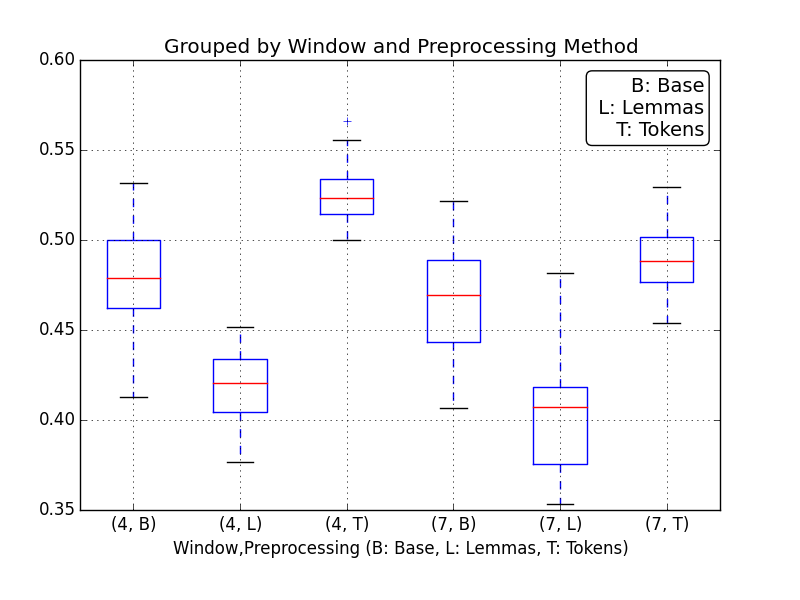
\includegraphics[width=\linewidth]{results_spearman/ar_similiarity_task_results_ws353_spearplot.png}
  \caption{Results on Arabic Word Similarity 353}
  \label{fig:spearplotws353}
\end{figure}

\section{Our Similarity Task}

Tables \ref{table:ourtask}, \ref{table:ourtaskmulti}, and \ref{table:ourtask4} show the results of the models with the 10 highest correlation scores on the task we developed. Each table displays results on different subsets of our data, selected by the minimum number of fluent Arabic evaluators that contributed labels to the word pairs. These subsets are the collections where each word pair has at least one evaluator, at least two evaluators, and at least four evaluators (maximum is four). These results all demonstrate similar trends in Figures \ref{fig:spearplot1}, \ref{fig:spearplot2}, and \ref{fig:spearplot4}. The Kendall Tau scores between these three rankings are .335 between the full set of word pairs and the set with four votes, .482 between the full set and the set with two or more votes, and .572 between the task with two votes and the task with four votes (all highly significant). Tables \ref{table:ourtask}, \ref{table:ourtaskmulti}, and \ref{table:ourtask4} do demonstrate that with more evaluators, the models become better correlated with the task. Interestingly, the base Arabic without tokenization or lemmatization produces the highest correlation scores on our task. This observation, along with the improvements with more voters, suggests that as our task draws the most common words from the same Wikipedia corpus that the models are trained on, the embeddings are able to directly learn the semantic similarity of these base words without the aid of lemmatization or tokenization. As the word pair similarities become more correlated with the model as we add fluent evaluators, these results also suggest that the control model is able to predict a similarity score more consistently accurate than our human labelers, assuming that the similarity scores will converge to a true label as we add human labelers. Additionally, Figures \ref{fig:spearplot1}, \ref{fig:spearplot2}, and \ref{fig:spearplot4} support our findings that the smaller window size does indeed have a strong positive impact on the quality of the word embeddings.

% full/4: tau: 0.334649122807, p_value: 1.36433095045e-06
% multi/full: tau: 0.481578947368, p_value: 3.63086505503e-12
% multi/4: tau: 0.572368421053, p_value: 1.44144439867e-16

% Embedding File,MSE,Accuracy,Hit_Percent,Correlation,Correlation Sig,Spearman,Spearman Sig,wind,size,mod,dig,tash,preprocessing
% 1              2    3        4            5          6           7    8        9           10   11   12  13  14   15

\begin{table}
\begin{center}
\begin{tabular}{l|l|l|l|l}
\bfseries Rank & \bfseries Preprocessing & \bfseries Window & \bfseries Size & \bfseries Correlation
\csvreader[head to column names]{results_spearman/ar_similiarity_task_results_prepared.csv}{}
{\\\hline\rank&\preprocessing&\wind&\size&\Spearman}
\end{tabular}
\caption{Top Results on our whole Arabic Task}
\label{table:ourtask}
\end{center}
\end{table}

\begin{table}
\begin{center}
\begin{tabular}{l|l|l|l|l}
\bfseries Rank & \bfseries Preprocessing & \bfseries Window & \bfseries Size & \bfseries Correlation
\csvreader[head to column names]{results_spearman/ar_similiarity_task_multi_results_prepared.csv}{}
{\\\hline\rank&\preprocessing&\wind&\size&\Spearman}
\end{tabular}
\caption{Top Results on our Arabic Task - 2+ Votes}
\label{table:ourtaskmulti}
\end{center}
\end{table}

\begin{table}
\begin{center}
\begin{tabular}{l|l|l|l|l}
\bfseries Rank & \bfseries Preprocessing & \bfseries Window & \bfseries Size & \bfseries Correlation
\csvreader[head to column names]{results_spearman/ar_similiarity_task_4_votes_results_prepared.csv}{}
{\\\hline\rank&\preprocessing&\wind&\size&\Spearman}
\end{tabular}
\caption{Top Results on our Arabic Task - 4 Votes}
\label{table:ourtask4}
\end{center}
\end{table}

\begin{figure}
  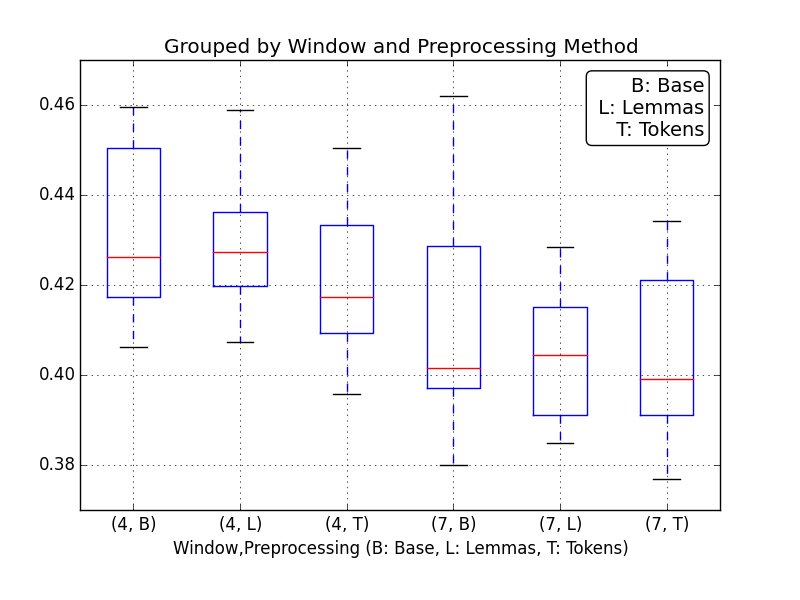
\includegraphics[width=\linewidth]{results_spearman/ar_similiarity_task_results_spearplot.png}
  \caption{Results on Our Whole Arabic Task}
  \label{fig:spearplot1}
\end{figure}

\begin{figure}
  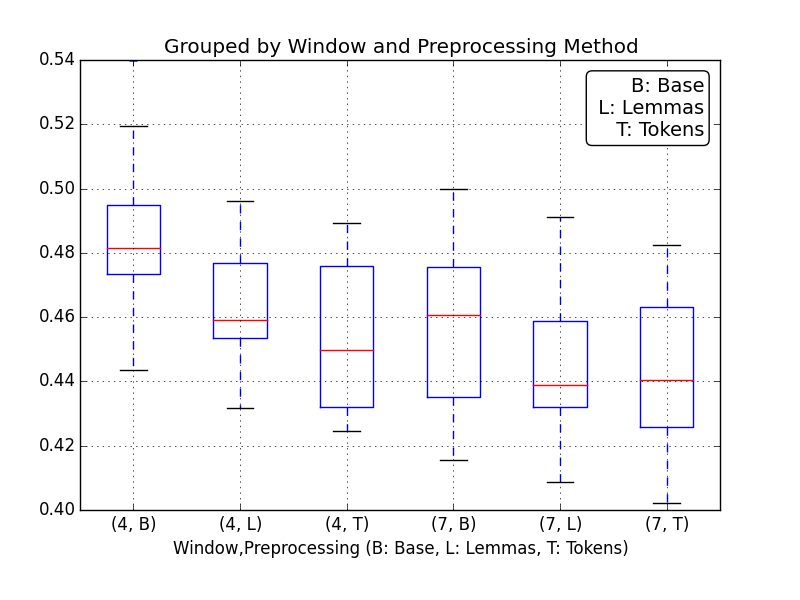
\includegraphics[width=\linewidth]{results_spearman/ar_similiarity_task_multi_results_spearplot.png}
  \caption{Results on Our Arabic Task - 2+ Votes}
  \label{fig:spearplot2}
\end{figure}

\begin{figure}
  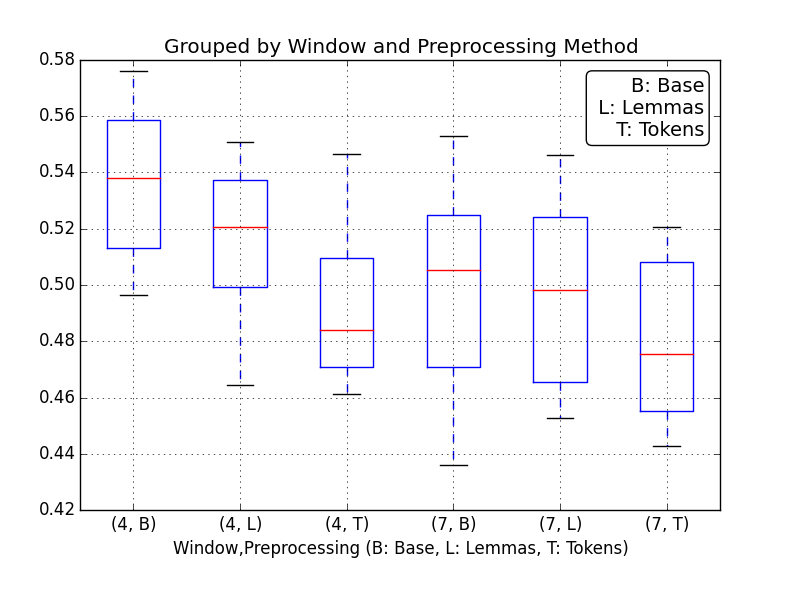
\includegraphics[width=\linewidth]{results_spearman/ar_similiarity_task_4_votes_results_spearplot.png}
  \caption{Results on Our Arabic Task - 4 Votes}
  \label{fig:spearplot4}
\end{figure}



These similarity task experiments have shown that certain preprocessing and training decisions can substantially change the performance of Arabic word embeddings on similarity tasks. Some choices did not demonstrate any significant impact on any of our results, such as choosing between CBOW and Skip Gram algorithms. Some methods were able to surpass the English baseline. While the best performing models were still significantly below the scores of the English embeddings trained on the Google News corpus, this is to be expected considering the strong correlation between the quantity of training data and the quality of the word embeddings, and our training set has approximately 5 million Arabic words while the Google News set has about 100 billion words \cite{mikolovdist:2013}.

\section{Analogy Task}

Table \ref{table:englishanalogy} shows the baseline results of the English embeddings on the Analogy task. These results demonstrate the extreme difference in quality between vectors trained on 5 million words and 100 billion words. The lower accuracy of the 5 million word model at $0.04522$, or 4.522 percent correct of the $19544$ analogies, will be used as a comparitive baseline for this task. We leave trying a larger model as future work.


\begin{table}
\begin{center}
\begin{tabular}{l|l}
\bfseries Model & \bfseries Accuracy
\csvreader[head to column names]{results_analogy/en_prepared.csv}{}
{\\\hline\csvcoli&\csvcoliii}
\end{tabular}
\caption{English Analogy Results}
\label{table:englishanalogy}
\end{center}
\end{table}

% Embedding File,Hit_Percent,Scores,wind,size,mod,dig,tash,preprocessing
% 1               2           3      4   5      6 7    8   9

Table \ref{table:aranalogy} shows the top 10 analogy task results from the Arabic models. Here it seems models preprocessed to lemmas and trained to 200 dimensions seem to dominate. We also see less difference between models with different window sizes. Figure \ref{fig:aranalogy} confirms these trends with boxplots with groups by significant factors. This plot illustrates the dramatic improvements that are obtained with proper preprocessing and parameterization for the task. The lemmatized 200 dimensional models consistently outperformed all other models, including the baseline English model. In the best case, one ideally parameterized model is nearly 50\% better than the English baseline. Of lesser note, the tokenization method also delivers significantly higher accuracies than the models that received no preprocessing on the Arabic. These results demonstrate that preprocessing and training decisions can greatly improve the performance of Arabic word embeddings on analogy solving tasks, improving scores from as low as half of the English baseline to as high as 150\% of the baseline.

\begin{table}
\begin{center}
\begin{tabular}{l|l|l|l|l}
\bfseries Rank & \bfseries Preprocessing & \bfseries Window & \bfseries Size & \bfseries Accuracy
\csvreader[head to column names]{results_analogy/ar_analogy_results_fixed_prepared.csv}{}
{\\\hline\rank&\csvcolix&\csvcoliv&\csvcolx&\csvcoliii}
\end{tabular}
\caption{Top Results on Arabic Analogy Task}
\label{table:aranalogy}
\end{center}
\end{table}

\begin{figure}
  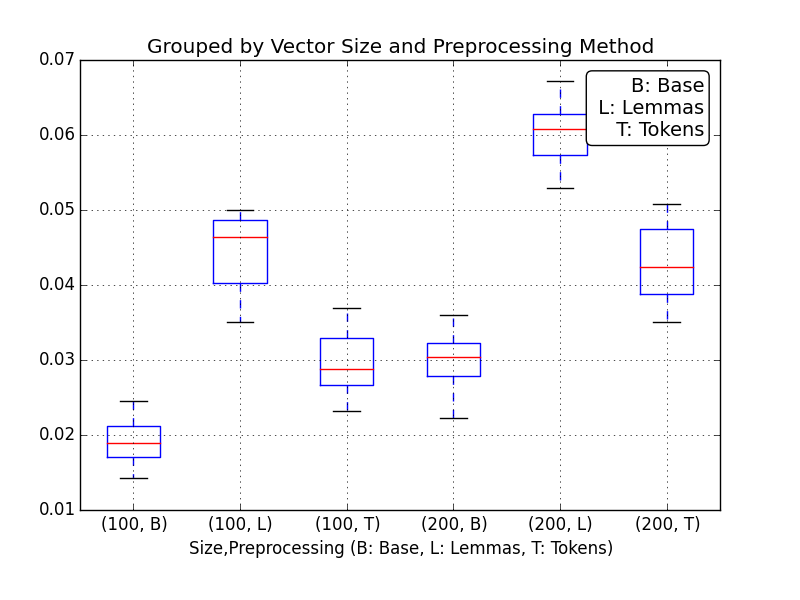
\includegraphics[width=\linewidth]{results_analogy/ar_analogy_results_fixed_plot.png}
  \caption{Arabic Analogy Task Results}
  \label{fig:aranalogy}
\end{figure}



















\bibliography{arabic-research}
\bibliographystyle{acl}
% \bibliographystyle{acl2016}

% \appendix

\end{document}
